\chapter{Preliminary Sizing}
\label{ch:PrelimSizing}
An iterative tool is developed for preliminary sizing to estimate several characteristics of the different concepts.
The tool consists of four main parts: the class I sizing in \Cref{sec:classI_sizing}, using wing and power loading diagrams; the class II sizing in \Cref{sec:Class_II_sizing}, calculating masses of (sub-)systems; the wing loading model in \Cref{sec:wing-loading}, calculating the shear and bending loads on the hinges; and the noise model in \Cref{sec:noise_model}, calculating the noise levels of the different concepts.

An overview of the preliminary sizing tool and the manner of how different models interact with each other can be seen in \Cref{fig:prelim_sizing_flow}.
The preliminary sizing from the Class I estimation (\Cref{sec:classI_sizing}) can be used to generate a Class II sizing.
Where Class II sizing is an iterative process that calculates the mass of the different components of the vehicle.
The mass of the energy system, airframe, propulsion system, and payload are calculated separately and summed up to get an updated total mass.
The updated total mass is then compared with the estimation from Class I, if the absolute difference is bigger than some tolerance ($\epsilon=10^{-6}$ is used) the Class I sizing will be reiterated.
Subsequently, the iterated class I sizing is used to reiterate the class II sizing.

After the Class I-II iteration, parameters like wing dimension, takeoff power, total mass, and sub-masses are set.
These parameters are used in the wing loading model (\Cref{sec:wing-loading}) to calculate the shear and bending loads on the hinges, as well as for the noise model (\Cref{sec:noise_model}) to calculate the noise levels of the different concepts.

From the outputs of the preliminary sizing, mass breakdown (\Cref{fig:mass-breakdown}), energy breakdown (\Cref{fig:energy-breakdown}), and wing loading diagrams (\Cref{fig:WPWS-diagrams}) are generated for each concept.
These diagrams are presented and discussed in \Cref{sec:sizing-results}.

The details of the in- and outputs of the different models and functions inside the preliminary sizing tool can be seen in \Cref{fig:prelim_sizing_N2}. %\todo{this reference does not seem to work, idk what is happening}

In the preliminary sizing, multiple assumptions have been made to simplify the calculations, which are discussed in the following sections.
Certain aspects of the different concepts, like hinge masses, a possible backup generator, and emergency rerouting, are not considered in the preliminary sizing.
These assumptions and ignored aspects influence the accuracy of the results.
However, this influence is expected to be equal for all concepts and, therefore, still valid for the trade-off in \Cref{ch:TradeOff}.

\begin{figure}[h!]
    \centering
    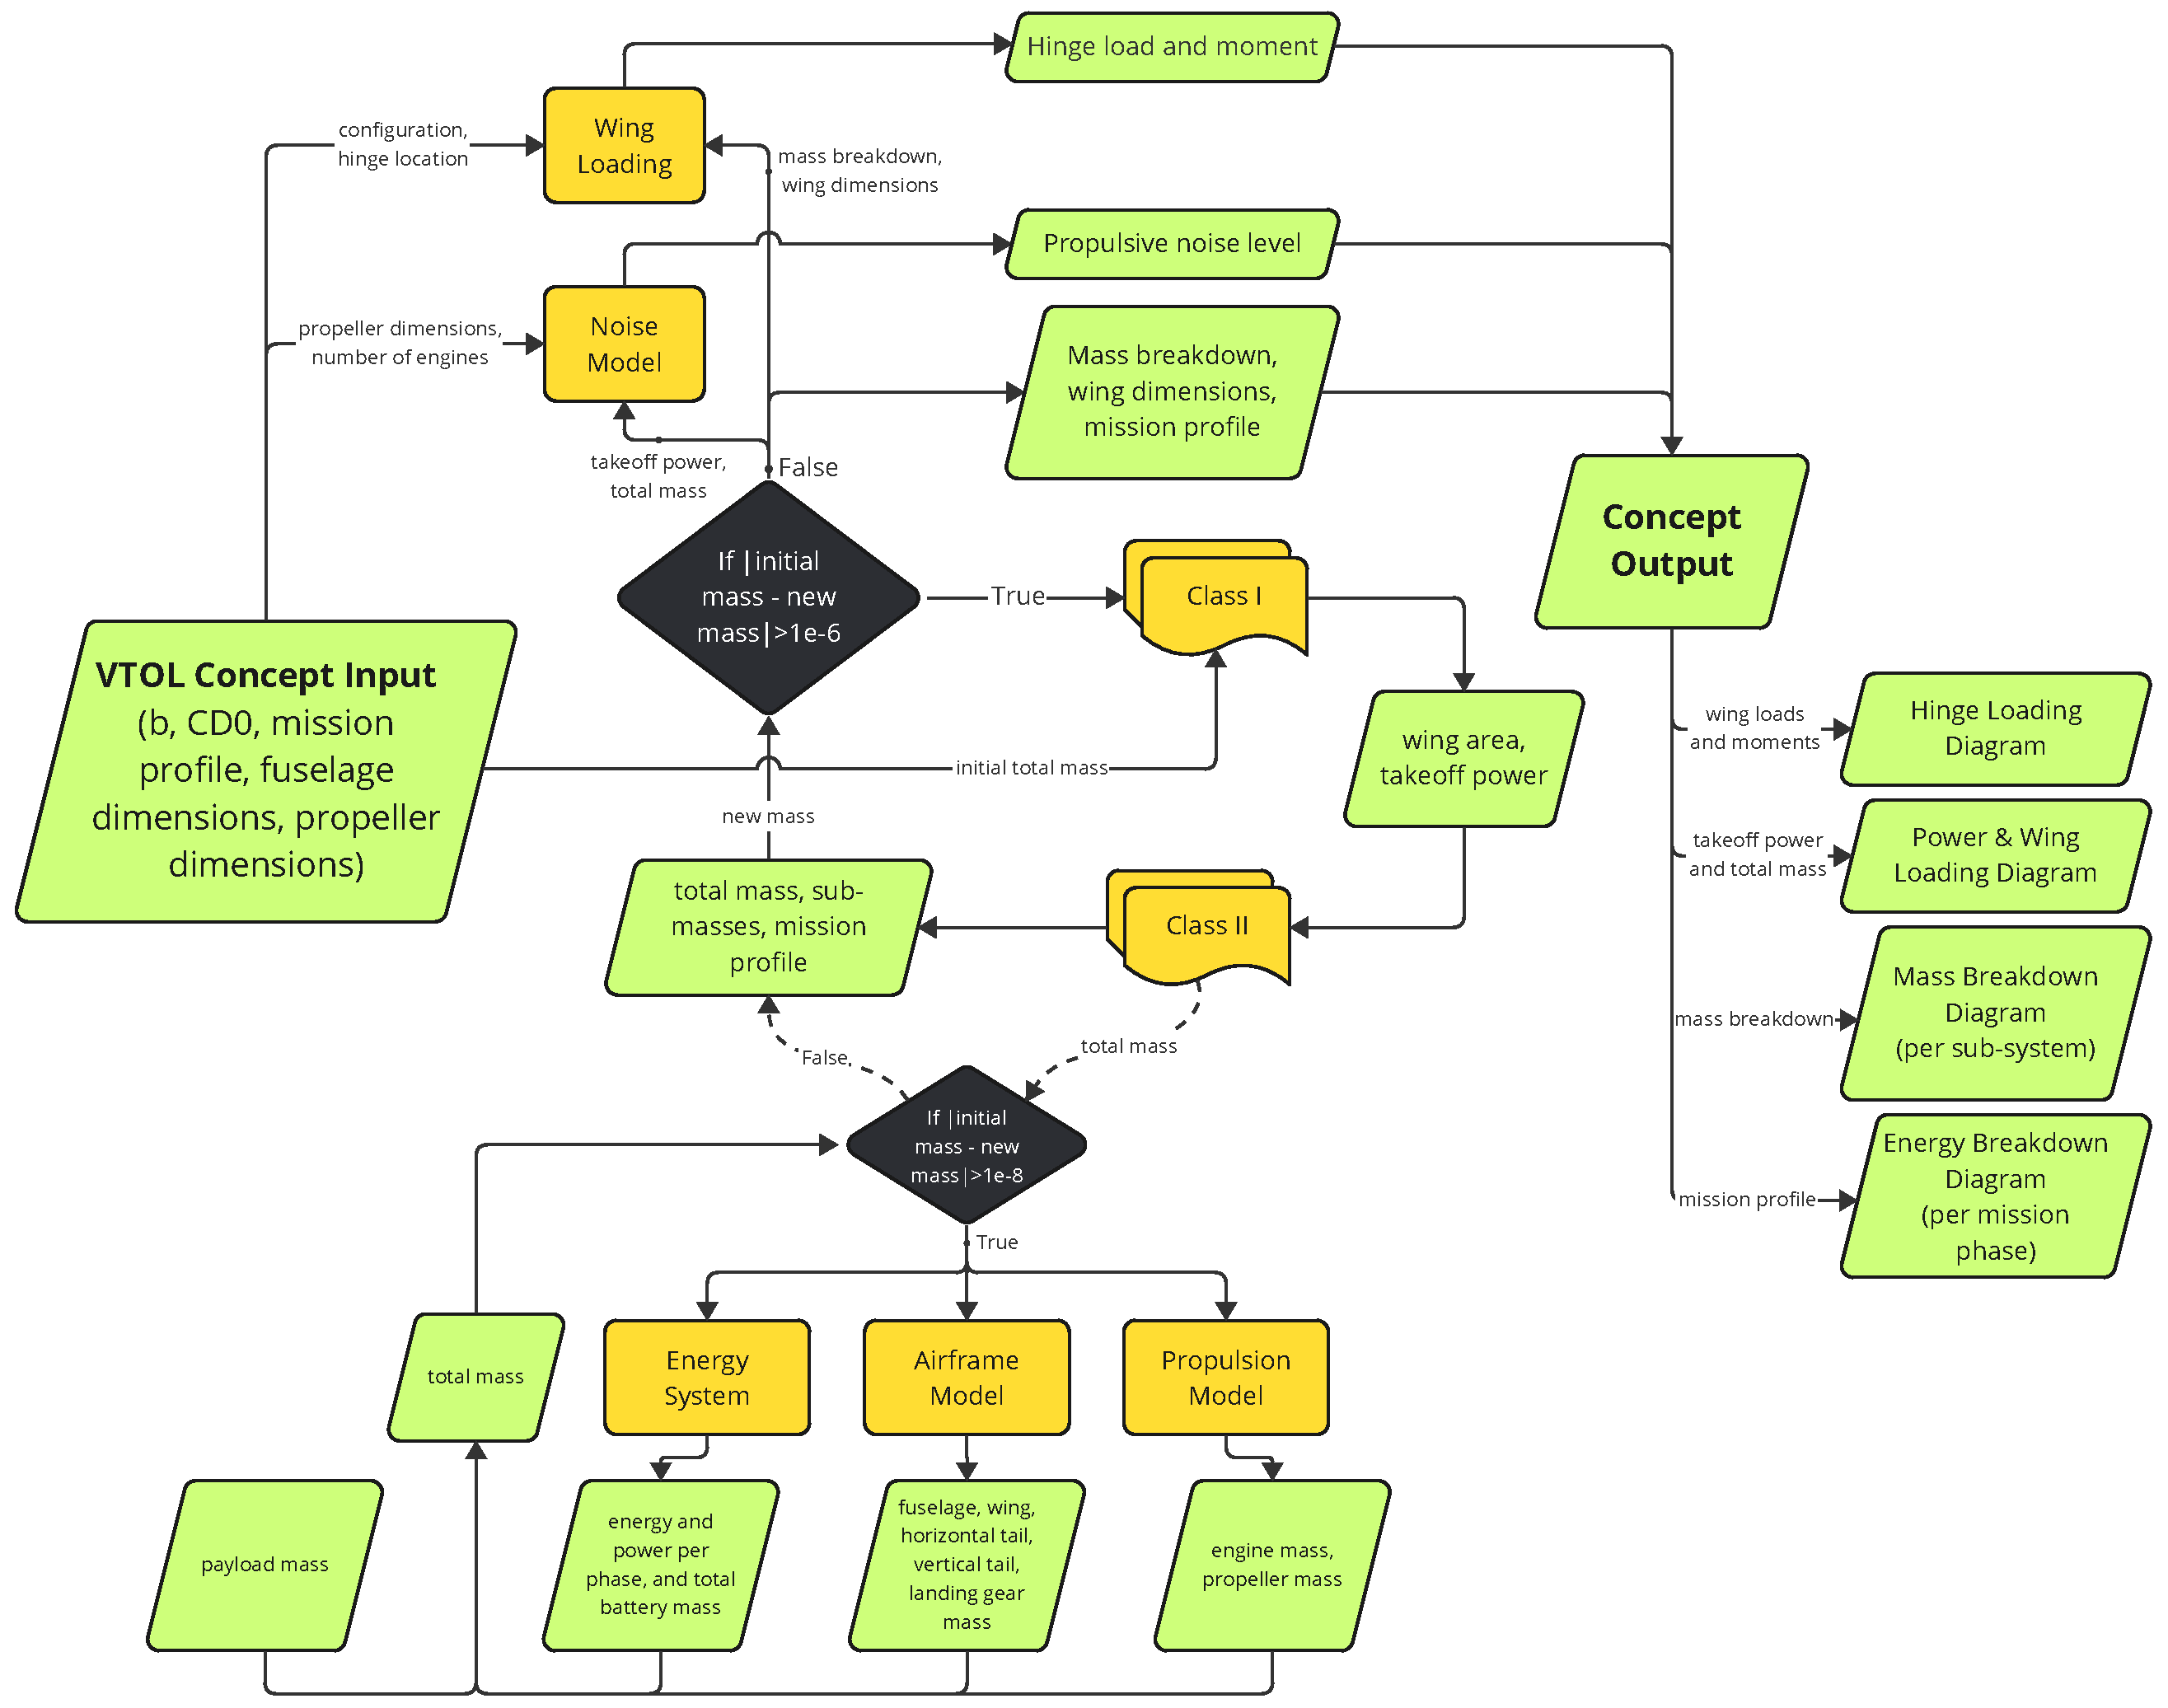
\includegraphics[width=\linewidth]{figures/PreliminarySizing/PreliminarySizingFlow}
    \caption{Flowchart of the preliminary sizing model}
    \label{fig:prelim_sizing_flow}
\end{figure}

\begin{figure}[H]
    \centering
    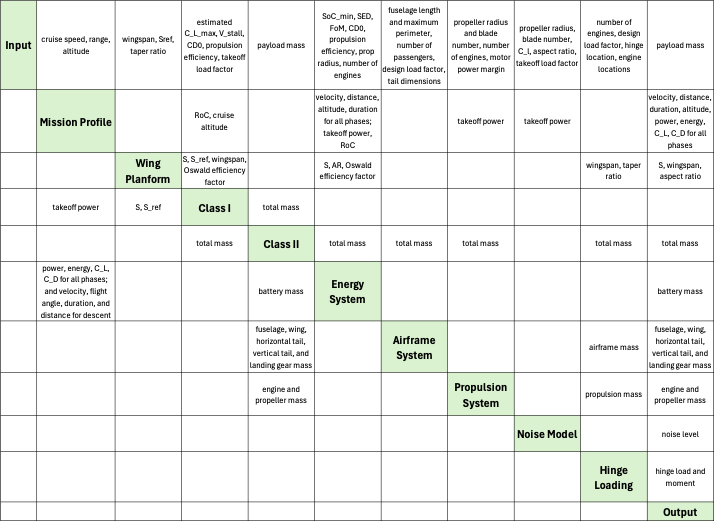
\includegraphics[width=\linewidth]{figures/PreliminarySizing/SizingN2}
    \caption{N2 chart of in- and outputs of functions in the preliminary sizing model}
    \label{fig:prelim_sizing_N2}
\end{figure}


\section{Wing and Power Loading}\label{sec:classI_sizing}
The first step in the preliminary sizing is the construction of the wing loading (W/S) and power loading (W/P) diagrams.
These diagrams depend on the total weight of the eVTOL, which is initially estimated by regression of data of competitor eVTOLS. Using this mass, an initial wing and power sizing can be performed, which can be further iterated in Class II sizing \Cref{sec:Class_II_sizing}.

The loading diagram contains the wing and power loading during different mission phases, which have been split up into takeoff, climb and cruise.
The landing phase is assumed to be similar and less constraining than the takeoff phase.

\subsection{Loading Diagrams Phases}

\subsubsection{Take-off}
During takeoff, the vehicle will travel vertically, which gives a constraint on the power loading.
The thrust needed to take off vertically was calculated to be $   T = W + D$, where the weight ($W$) was initially estimated by literature and the drag ($D$) can be calculated in \Cref{eq:vertical thrust}.
\begin{equation}
    \label{eq:vertical thrust}
    T = W_{\text{total}} +\frac{1}{2}\cdot\rho\cdot(\text{RoC})^2_{\text{VTOL}}\cdot S_{\text{ref}}\cdot C_{\text{D}}
\end{equation}
$C_{\text{D}}$ was estimated by the assumption of flat plate drag, which is valid since the aircraft acts as a flat plate during vertical ascent, using \Cref{eq:Cdvertical}~\cite{prelimSizingLoadingdiagram}.
\begin{equation}
    \label{eq:Cdvertical}
    C_{\text{D}_{\text{vertical}}} = 2\cdot \sin^3(\alpha)
\end{equation}
 Since the angle of attack $\alpha$ is 90 degrees, $C_{\text{D}}$ equals 2. $S_{\text{ref}}$ is the frontal reference area of the vehicle, $\rho$ is the air density at take-off altitude and (RoC) is the vertical rate of climb, which is assumed to be 5 m/s.
Using these values, the thrust-over-weight ratio can be computed for a vertical climb, as can be seen in \Cref{eq:T//2 vertical climb}.
\begin{equation}
    \label{eq:T//2 vertical climb}
    \frac{T}{W} = n_{\text{load}}\left(1+ \frac{1}{W/S}\rho (\text{RoC})^2 \frac{S_{\text{ref}}}{S}\right)
\end{equation}
Where $W$ is the aircraft's total weight, and $S$ is the wing's surface area.
 An extra load factor, $n_{\text{load}}$ is assumed to be 1.2~\cite{prelimSizingLoadingdiagram}.
This 20 $\%$ extra thrust accounts for trim and wind gusts.

To convert this ratio to power loading, the following relationship was used, expressed in \Cref{eq:powerloadingvtol}:
\begin{equation}
    \label{eq:powerloadingvtol}
    \frac{W}{P}_{\text{VTO}} = \left(\frac{T}{W}\cdot \sqrt{\frac{T/A}{2\cdot \rho}}\right)^{-1} \cdot \text{FM} \cdot\eta_{\text{prop}}
\end{equation}
In \Cref{eq:powerloadingvtol}, FM is the Figure of Merit, which can be seen as the rotor efficiency.
Moreover, the $T/A$ is the disk loading and is calculated by the total thrust divided by the total rotor disk area. Finally the $\eta_{\text{prop}}$ is the propulsive efficiency and is taken as 0.85 from the Joby S4 \cite{moller2020performance}.

\subsubsection{Climb}
After the vertical takeoff, the vehicle starts a climb.
During this climb, an initial rate of climb (RoC) was assumed to be \qty{5}{m/s}.
The $\frac{C_{\text{D}}}{C_{\text{L}}^{3/2}}$ term should be optimal for an optimal climb and therefore a minimum value~\cite{ADSEEIslides}.
The density is set at the cruise altitude since the climb endures until the cruise. Based on these assumptions \Cref{eq:climb} is constructed
\begin{equation}
    \label{eq:climb}
    \frac{W}{P}_{\text{cruise}} = \left(  \operatorname{RoC} +  \left( \frac{2W/S}{\rho}\right)^{(1/2)} \cdot  \left( \frac{C_{\text{D}}}{C_{\text{L}}^\frac{3}{2}}\right )_{\text{opt}} \right)^{-1} \cdot  \eta_{\text{prop}}
\end{equation}

\subsubsection{Cruise}
The power loading for the cruise is determined at an altitude of   \qty{500}{m}.
This is used in the $\rho/\rho_{0}$ to account for air density.
Furthermore, the 2-term drag polar is used to describe the drag in which the lift is equal to the weight.
Hence, the final equation can be seen in \Cref{eq:WPcruise}. Where $AR$ is the aspect ratio, $e$ is the Oswald efficiency factor and $C_{\text{D}_{0}}$ is the drag coefficient when the wing produces no lift.
\begin{equation}
    \label{eq:WPcruise}
    \frac{W}{P}_{\text{cruise}} = \eta_{prop} \cdot  \left( \frac{\rho}{\rho_{0}} \right )^{3/4} \left ( \frac{C_{\text{D}_{0}}\cdot \frac{1}{2}\rho V^3} {W/S} + \left( \frac{W}{S} \right) \frac{1}{\pi AR e \frac{1}{2} \rho V} \right) ^{-1}
\end{equation}

\subsubsection{Stall}
The vehicle can stall during cruise or transition, hence constraining the diagram vertically.
The stall speed ($V_{\text{stall}}$) is taken from the CS23 requirement for a small aircraft and taken as \qty{32}{m/s}~\cite{easa_cs23_2020}. Thus, the wing loading for stall speed can be determined using \Cref{eq:stall} where $C_{\text{L}_{\max}}$ is the maximum lift coefficient.
\begin{equation}
    \label{eq:stall}
    \frac{W}{S}_{\text{stall}} = 0.5\cdot \rho\cdot C_{\text{L}_{\max}}\cdot V_{\text{stall}}^2
\end{equation}

The wing loading and power loading diagrams can be constructed from these equations.
They are constructed for all four concepts that differ in geometry, resulting in the final graphs in \Cref{fig:WPWS-diagrams} in \Cref{sec:sizing-results}.


From these figures, the design points can be calculated, and using an initial mass estimation, the initial span and power can be obtained.
These values are the inputs for the class II sizing method from which the iteration starts.


\section{Class II Sizing}
\label{sec:Class_II_sizing}
The class II method that will be used is by Ugwueze et al.~\cite{Ugwueze_Sizing_Method}, the described method uses the Cessna method from Roskam~\cite{Roskam_Part_V}.
As can be seen in \Cref{eq:m_total_classII,eq:m_empty_classII}, the empty mass is split up into the energy system mass ($m_\text{b}$), airframe mass ($m_\text{a}$) and the propulsion system mass ($m_\text{p}$).
The three sub-masses are calculated separately, as will be discussed in \Cref{subsec:Class_II_sizing_Energy_System_Mass,subsec:Class_II_sizing_Airframe_Mass,subsec:Class_II_sizing_Propulsion_System_Mass} and summed up to get the total empty mass.

The calculations for the sub-masses depend on the total mass, $m$.
Thus, the Class II mass estimation is iterated until the difference between the total mass and the sum of the sub-masses is smaller than some tolerance, $\epsilon=10^{-8}$, as can be seen in \Cref{fig:prelim_sizing_flow}.


\begin{minipage}{.45\linewidth}
    \begin{equation}
    \label{eq:m_total_classII}
    m = m_{\text{empty}} + m_{\text{payload}}
\end{equation}
\end{minipage}
~
\begin{minipage}{.45\linewidth}
    \begin{equation}
    \label{eq:m_empty_classII}
    m_{\text {empty }}=m_\text{b}+m_\text{a}+m_\text{p} 
\end{equation}
\end{minipage}




\subsection{Energy System Mass}\label{subsec:Class_II_sizing_Energy_System_Mass}
The power is estimated for each phase of the mission profile to calculate the mass of the vehicle's battery.
By multiplying the power with the phase duration, the energy per phase can be calculated.
The energy per phase is then summed up to get the total energy needed for the mission profile.
From the total energy, the mass of the battery can be calculated using, i.e.\ the energy density of the battery.

The power per phase, with $P_{\text{hv}}$ the power required for hovering, $P_{\text{to}}$ the power for takeoff, $P_{\text{cl}}$ the climb power in vertical configuration, $P_{\text{cr}}$ the power for cruise, $P_{\text{desc}}$ the power for descend, and $P_{\text{ld}}$ the power required for landing, is computed with the following formulae~\cite{Ugwueze_Sizing_Method}:


\begin{minipage}{.45\linewidth}
\begin{equation}
\label{eq:ClassII_power_takeoff}
    P_{\text{to}} = P_{\text{hv}} 
\end{equation}
\end{minipage}
~
\begin{minipage}{.45\linewidth}
\begin{equation}
\label{eq:ClassII_power_hovering}
    P_{\text{hv}} = \frac{T^\frac32}{\operatorname{FM}\sqrt{2\rho A}} 
\end{equation}
\end{minipage}

\begin{minipage}{.45\linewidth}
\begin{equation}
\label{eq:ClassII_power_climb}
    P_{\text{cl}} = P_{\text{hv}} + \left( \frac{\operatorname{RoC}}{2v_{\text{hv}}} \sqrt{\left( \frac{\operatorname{RoC}}{2v_{\text{hv}}} \right)^2 + 1} \right) 
\end{equation}
\end{minipage}
~
\begin{minipage}{.45\linewidth}
\begin{equation}
\label{eq:ClassII_power_cruise}
    P_{\text{cr}} = \frac{1}{\eta_{\text{prop}}} \cdot \frac12 \rho V_{cr}^3 S \left( C_{\text{D}_0} + \frac{C_{\text{L}_{\text{cr}}}^2}{\pi AR\cdot e} \right) \\
\end{equation}
\end{minipage}

\begin{minipage}{.45\linewidth}
\begin{equation}
\label{eq:ClassII_power_descend}
    P_{\text{desc}} = 0
\end{equation}
\end{minipage}
~
\begin{minipage}{.45\linewidth}
\begin{equation}
\label{eq:ClassII_power_landing}
    P_{\text{ld}} = 0
\end{equation}
\end{minipage}   




% \begin{align}
%     P_{\text{hv}} &= \frac{T^\frac32}{\operatorname{FM}\sqrt{2\rho A}} \\
%     P_{\text{to}} &= P_{\text{hv}} \\
%     P_{\text{cl}} &= P_{\text{hv}} + \left( \frac{\operatorname{RoC}}{2v_{\text{hv}}} \sqrt{\left( \frac{\operatorname{RoC}}{2v_{\text{hv}}} \right)^2 + 1} \right) \\
%     P_{\text{cr}} &= \frac{1}{\eta_{\text{prop}}} \cdot \frac12 \rho V_{cr}^3 S \left( C_{\text{D}_0} + \frac{C_{\text{L}_{\text{cr}}}^2}{\pi AR\cdot e} \right) \\
%     P_{\text{desc}} &= 0 \\
%     P_{\text{ld}} &= 0
% \end{align}

With the disk thrust, $T=W_{\text{tot}}$, total weight, $W_{\text{tot}}=mg$, total mass, $m$, figure of merit, $\operatorname{FM}=0.75$, disk area, $A=2\pi r_{\text{prop}}^2n_{\text{prop}}$, propeller radius, $r_{\text{prop}}$, number of propellers, $n_{\text{prop}}$, air density, $\rho(h)$, altitude, $h$, wing area, $S$, rate of climb, $\operatorname{RoC}=\qty{5}{\m\per\s}$, hover velocity, $v_{\text{hv}}=P_{\text{hv}}/T$, propeller efficiency, $\eta_{\text{prop}}=0.85$, cruise velocity, $V_{cr}=\qty{200}{\km\per\hour}$,  zero-lift drag coefficient, $C_{\text{D}_0}$, the lift coefficient, $C_{\text{L}_{\text{cr}}}=\frac{2W_{\text{tot}}}{\rho V_{cr}^2 S}$, aspect ratio, $AR$, and Oswald efficiency factor, $e=0.85$.

The energy per phase, $E_{\text{ph}}$, is then calculated by multiplying the power per phase with the duration of the phase, $t_{\text{ph}}$ see \Cref{eq:phasepow}. With the energy per phase, the total energy, $E_{\text{tot}}$, is calculated by summing up the energy per phase as seen in \Cref{eq:totpow}:

\begin{minipage}{.45\linewidth}
\begin{equation}
\label{eq:phasepow}
    E_{\text{ph}} = P_{\text{ph}} \cdot t_{\text{ph}}
\end{equation}
\end{minipage}
~
\begin{minipage}{.45\linewidth}
\begin{equation}
    \label{eq:totpow}
    E_{\text{tot}} = \sum_{i=1}^{n} E_{\text{ph}_i}
\end{equation}
\end{minipage}

A minimum battery state of charge ($\operatorname{SoC}_{\min}=20\%$) is set to ensure the longevity of the battery and to provide an extra energy reserve for emergencies~\cite{Ugwueze_Sizing_Method}.
The battery mass, $m_b$, is then calculated from the total energy of the mission~\cite{Ugwueze_Sizing_Method}:
\begin{equation}
    m_b = \frac{E_{\text{tot}}(1+\operatorname{SoC}_{\operatorname{min}})}{\operatorname{SED}\cdot\eta_{\text{bat}}}
\end{equation}
With the specific energy density of the battery, $\operatorname{SED}=\qty{300}{\watt\hour\per\kilo\gram}$, and the battery efficiency, $\eta_{\text{bat}}=0.85$.

\subsection{Airframe Mass}
\label{subsec:Class_II_sizing_Airframe_Mass}

\Cref{eq:m_fuselage_classII,eq:m_wing_classII,eq:m_horizontal_tail_classII,eq:m_vertical_tail_classII} are empirical formulas taken from the Cessna class II method of Roskam~\cite{Roskam_Part_V}, while \Cref{eq:m_landing_gear_classII} is taken from the USAF method of Roskam~\cite{Roskam_Part_V}.

\begin{equation}
    \label{eq:m_fuselage_classII}
    m_f=14.86 m^{0.144}{\frac{l_f}{P_{\max }}}^{0.778} l_f^{0.383} N_{\text{pax}}^{0.455}
\end{equation}
In \Cref{eq:m_fuselage_classII} $m_f$ is the fuselage mass in \unit[]{lbs}, $m$ is the takeoff mass in \unit[]{lbs}, $l_f$ is the length of the fuselage without the nose-mounted nacelle in \unit{ft}, $P_{\max}$ is the maximum fuselage perimeter in \unit{ft} and $N_{\text{pax}}$ is the number of passengers.


\begin{equation}
    \label{eq:m_wing_classII}
    m_w=0.04674 m^{0.397} S_w^{0.360} \eta_w{ }^{0.397} \mathrm{AR}_w^{1.712}
\end{equation}
\Cref{eq:m_wing_classII} holds for cantilever wings, $m_w$ is the mass of the wing in \unit[]{lbs}, $S_w$ is the wing area in \unit[]{ft^2}, $\eta_w{ }$ is the design ultimate load factor and $\mathrm{AR}_w$ is the aspect ratio of the wing.


\begin{equation}
    \label{eq:m_horizontal_tail_classII}
    m_{t, h}  =\frac{3.184 m^{0.887} S_{t, h}^{0.101} \mathrm{AR}_{t, h}^{0.138}}{174.04 t_{r, h}^{0.223}}
\end{equation}
In \Cref{eq:m_horizontal_tail_classII}, $ m_{t, h}$ is the mass of the horizontal tail in \unit[]{lbs}, $S_{t, h}$ is the horizontal tail area in \unit{ft^2}, $\mathrm{AR}_{t, h}$ is the horizontal tail aspect ratio and $t_{r, h}$ is the horizontal tail maximum root thickness in \unit{ft}.

\begin{equation}
    \label{eq:m_vertical_tail_classII}
    m_{t, v}  =\frac{1.68 m^{0.567} S_{t, v}^{1.249} A R_{t, v}^{0.482}}{639.95 t_{r, v}^{0.747}\left(\cos \Lambda_{0.25 t, v}\right)^{0.882}}
\end{equation}
In \Cref{eq:m_vertical_tail_classII}, $m_{t, v}$ is the mass of the vertical tail in \unit[]{lbs}, $S_{t, v}$ is the vertical tail area in \unit{ft^2}, $\mathrm{AR}_{t, v}$ is the vertical tail aspect ratio, $t_{r, v}$ is the vertical tail maximum root thickness in \unit{ft} and $\Lambda_{0.25 t, v}$ is the vertical tail quarter chord's sweep angle.

\begin{equation}
    \label{eq:m_landing_gear_classII}
    m_{l g}=0.054 l_{l g}{ }^{0.501}\left(m\cdot\eta_{l g}\right)^{0.684}
\end{equation}
In \Cref{eq:m_landing_gear_classII}, $m_{l g}$ is the mass of the landing gear in \unit[]{lbs}, $l_{l g}$ is the strut length of the landing gear in \unit{ft} and $\eta_{l g}$ is the landing gear design load factor.

The total mass of the airframe, $m_a$, is the sum of the masses of the fuselage, wing, horizontal tail, vertical tail and landing gear:
\begin{equation}
    \label{eq:m_airframe_classII}
    m_a = m_f + m_w + m_{t, h} + m_{t, v} + m_{l g}
\end{equation}
The masses from \Cref{eq:m_fuselage_classII,eq:m_wing_classII,eq:m_horizontal_tail_classII,eq:m_vertical_tail_classII,eq:m_landing_gear_classII} are in \unit{lbs}, hence the masses are converted to \unit{kg}.

\subsection{Propulsion System Mass}\label{subsec:Class_II_sizing_Propulsion_System_Mass}
The propulsion system mass is calculated using \Cref{eq:m_motor_classII,eq:m_prop_classII}~\cite{Ugwueze_Sizing_Method,torenbeek_1982}, where the motor mass, $m_{\text{mot}}$, is calculated using the empirical \Cref{eq:m_motor_classII}~\cite{Ugwueze_Sizing_Method}:
\begin{equation}
    \label{eq:m_motor_classII}
    m_{\text{mot}}=0.165 \frac{P_{\max} (1+\operatorname{PM})}{n_{\text{mot}}}
\end{equation}
With the maximum power, $P_{\max}$ in \unit{kW}, the power margin, $\operatorname{PM}=0.5$, and the number of engines, $n_{\text{mot}}$.
The propeller mass, $m_{\text{prop}}$, is calculated using the empirical \Cref{eq:m_prop_classII}~\cite{Ugwueze_Sizing_Method}:
\begin{equation}
    \label{eq:m_prop_classII}
    m_{\text{prop}}=0.144 \left( d_{\text{prop}} \frac{P_{\max}}{N_{\text{prop}}} N_{\text{bl}}^{0.5} \right)^{0.782}
\end{equation}
With the propeller diameter, $d_{\text{prop}}$, the number of propellers, $N_{\text{prop}}$, and the number of blades, $N_{\text{bl}}$.
As in \Cref{eq:m_empty_classII}, the total mass of the propulsion system is the sum of the masses of the motor and propeller:
\begin{equation}
    \label{eq:m_propulsion_classII}
    m_p = m_{\text{mot}} + m_{\text{prop}}
\end{equation}


\section{Mechanism Loading}\label{sec:wing-loading}
\label{sec:Hingeload}
An essential step of mechanism sizing is the identification of load cases and the estimation of the load magnitudes.
Before doing so, two main mechanism categories can be defined among the proposed concepts: mechanisms that facilitate wing movement and propulsion rotation.
In the first two subsections, the loading on these two categories is going to be further investigated.
Finally, the results of both analyses are presented.

\subsection{Wing Rotating and Folding Mechanism}
To begin the hinge load analysis, the wing moving mechanism was first considered.
This type of mechanism is responsible for the movement of the wing during the transition.
All four final concepts contain a wing mechanism, either a folding (\ref{C1.5},~\ref{C2.6}) or a rotating mechanism (\ref{C2.1},~\ref{C2.10}). The load case during the transition was not evaluated, as an insufficient amount of information was available for the transition of the different concepts.
Therefore, only the vertical takeoff and fixed-wing phases were analysed.

Firstly, the load cases in cruise conditions, as well as the lift and mass distribution, were examined, as these are present in all four concepts.
Due to the finite wing effect, the lift distribution is a function of the induced angle of attach and local chord length.
Since both depend on the precise geometry and structural design of the wing, an approximate trapezoid lift and mass distribution are assumed.
Furthermore, it is assumed that the net force acting on the wing is the difference between the total lift force and the design load factor times the wing weight.
This is approximately equal to the weight of the aircraft without the wing.
Subsequently, it is further assumed that both distributions are proportional to the local chord length.
The resulting load case is depicted on \Cref{fig:wing_fbd}.
As a result, \Cref{eq:internal_shear} and \Cref{eq:internal_moment} were given for the internal shear and bending moment respectively by~\cite{wingloading}.
\begin{align}
    \label{eq:internal_shear}
    &V(\eta) =  \frac{nW_{\text{fus}}}{b}\frac{2}{1+\lambda}\frac{b}{2}\left[ 1-\eta + \frac{1}{2}(\lambda-1)(1-\eta^2)\right]\\
    \label{eq:internal_moment}
    &M(\eta) =  \frac{nW_{\text{fus}}}{b}\frac{2}{1+\lambda}\frac{b^2}{4}\left[ 1-\eta - \frac{1}{2}(1-\eta^2)+\frac{1}{2}(\lambda-1)(1-\eta-\frac{1}{3}(1-\eta^3))\right]
\end{align}
Here $W_{\text{fus}}$ is the weight of the aircraft without the weight of the wing, $\lambda$ is the taper ratio, $b$ is the wingspan, $n$ is the load factor and $\eta \in [0;1]$ is the span-wise location, where the internal load is to be calculated.

\begin{figure}[h]
    \centering
    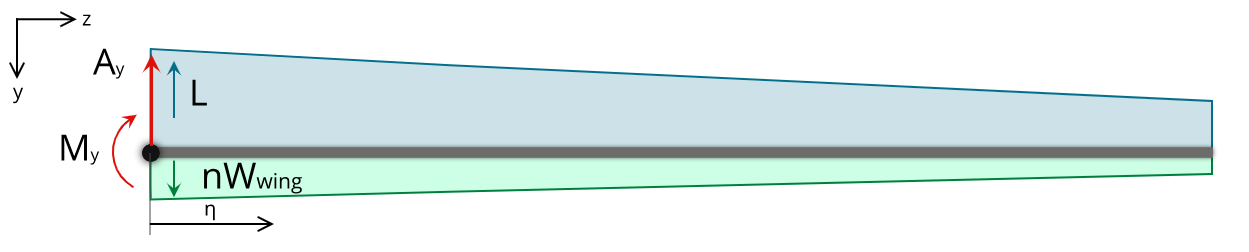
\includegraphics[width=\linewidth]{figures/PreliminarySizing/Wing_load_FBD.png}
    \caption{Wing and mass distribution over the wing}
    \label{fig:wing_fbd}
\end{figure}

Considering that some concepts have fuselage-mounted engines, the bending moment and shear force relief must be taken into account in the estimation.
The weight force of the engines is simulated as point forces; thus, the internal shear and moment of the wing due to purely two engines is placed at $l_1$ and $l_2$ from the root of the wing, given by \Cref{eq:internal_shear_engine} and \Cref{eq:internal_moment_engine}. Where $W_{\text{p}}$ is the weight of the propulsion unit.
\begin{align}
    \label{eq:internal_shear_engine}
    V(\eta)=-2nW_{\text{p}}, \ \eta \in [0;l_1]& & V(\eta)=-nW_{\text{p}}, \ \eta \in [l_1;l_2] & & V(\eta)= 0, \ \eta \in [l_2;1]
\end{align}
\begin{align}
    \label{eq:internal_moment_engine}
    M(\eta)=-\frac{nWb}{2}_{p}(l_1+l_2-2\eta), \ \eta \in [0;l_1]& & M(\eta)=-nW_{\text{p}}(l_2-\eta), \ \eta \in [l_1;l_2] & & M(\eta)= 0, \ \eta \in [l_2;1]
\end{align}
Combining the two loading types discussed above provides an approximate value for the internal bending moment and shear force at a chosen mechanism location.
Furthermore, loads in the XZ-plane are not considered, as the drag and thrust forces are expected to be less than the lift and weight.

Furthermore, the load cases during the hovering and vertical takeoff phases were investigated.
During these stages, the thrust point forces are applied to the wing, exposing the hinge to shear and bending.
However, this load case is only relevant to concept~\ref{C2.1} because it is the only design with a wing-mounted propulsion system, which lies after the hinge location with respect to the root.
This condition is presented on \Cref{fig:hover_fbd}, where the net thrust force equals the total weight times the design load factor.
The span-wise load distribution depicted on the FBD can be obtained by replacing the fuselage weight with purely the wing weight in \Cref{eq:internal_shear} and \Cref{eq:internal_moment} and combining with \Cref{eq:internal_shear_engine} \Cref{eq:internal_moment_engine}, taking into account the thrust force next to the propulsion weight.

\begin{figure}[h]
    \centering
    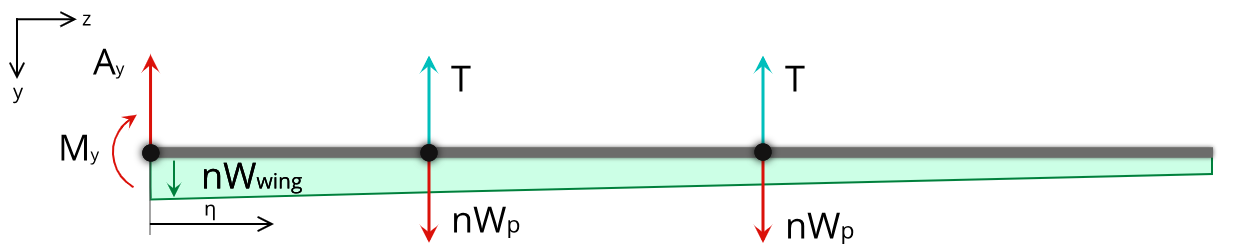
\includegraphics[width=\linewidth]{figures/PreliminarySizing/hover_wing_load_FBD.png}
    \caption{Free body diagram during hovering and vertical take-off}
    \label{fig:hover_fbd}
\end{figure}

\subsection{Propulsion Rotating Mechanism}
The subsequent type of mechanism is responsible for the reorientation of the propulsion system.
Conversely, in the previous analysis, only the folded scenario is considered, not the unfolded and the transition.
The rationale behind this decision is the higher loads during vertical takeoff since the thrust force has to be great enough to lift the weight of the vehicle.
As only the Winged Rotorcraft (\ref{C1.5}) and the Folding Wing (\ref{C2.6}) concepts have movable engines, the following analysis is only applicable to these vehicles.

To facilitate the ease of calculation, the following assumptions were taken:
Firstly, the centre of gravity coincides with the axis of the hinge, and it does not vary while functioning.
Furthermore, the line of action of the thrust force goes through the centre of gravity and intercepts the rotation axis of the mechanism.
Additionally, the mechanism of the Winged Rotorcraft concept is not placed in the fuselage but in the engine, resulting in a small moment arm that is considered zero at this stage of the design.
Contrarily, the Folding Wing concept has a rotating and translating engine, as depicted on \Cref{fig:engine_FBD}, meaning the moment arm $l$ cannot be neglected in this concept.

Utilising the aforementioned assumptions, the internal shear stress of the Winged Rotorcraft concept is given by \Cref{eq:engine_load1}.
The shear stress on the hinge of the Folding Wing concept is slightly higher than in the Winged Rotorcraft concept, as the force relief caused by the engine weight is not present.
This is because the hinge only lifts the propeller mass, which is negligible at this stage.
The internal shear force and moment of this concept are shown by \Cref{eq:engine_load2_shear,eq:engine_load2_moment}.

\begin{figure}
    \centering
        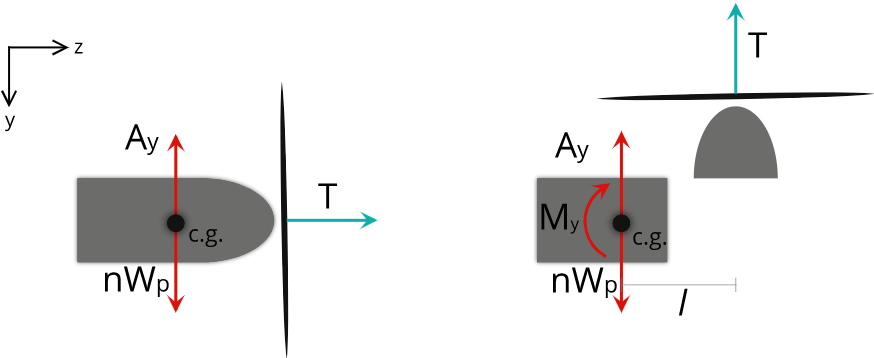
\includegraphics[width=0.5\linewidth]{figures/PreliminarySizing/engine_fbd.png}
        \caption{Free body diagram of the Folding Wing engine concept}
        \label{fig:engine_FBD}
\end{figure}

\begin{minipage}{.3\textwidth}
    \begin{equation}
    \label{eq:engine_load1}
    V = n\left(\frac{W_{\text{total}}}{4}W_{\text{p}}\right)
    \end{equation}
\end{minipage}
~
\begin{minipage}{0.3\textwidth}
    \begin{equation}
    \label{eq:engine_load2_shear}
        V = \frac{nW_{\text{total}}}{4}
    \end{equation}
\end{minipage}
~
\begin{minipage}{0.3\textwidth}
    \begin{equation}
    \label{eq:engine_load2_moment}
    M = \frac{nW_{\text{total}}l}{4}
    \end{equation}
\end{minipage}




\section{Noise Model}\label{sec:noise_model}
In order to estimate the noise generated by each concept, a noise model set up is presented in this section.
The model is based on the assumption that there are two main contributors to aircraft noise to be considered: engine noise and aerodynamic noise~\cite{aerodynamicKoutsoukos}, resulting from flow interactions.
Research shows that usually, 60\% of the overall aircraft noise is to be attributed to engine noise and 40\% to aerodynamic noise~\cite{noisepercentages}.
While propulsion noise will be numerically (quantitatively) discussed by means of the model presented in the paragraph below, aerodynamic noise will not be quantified in an absolute matter yet but only roughly estimated in \Cref{par:aeroscoring} for trade-off or comparison, purposes strictly.

\subsubsection{Propulsion Noise Model}
In order to get a quantitative
measure of propulsion noise, \Cref{eq:propnoise} is used~\cite{midtermnoise}.
\begin{equation}
\label{eq:propnoise}
    \mathrm{SPL}_{1, \max }=83.4+15.3 \log _{10} P_{\text{br}}-20 \log _{10} D+38.5 M_t-3(B-2)+10 \log _{10} N_p
\end{equation}
This equation gives the maximum sound pressure level in decibels (dB) at \qty{1}{m} from the source. $P_{\text{br}}$ is the engine power
in kW, $D$ is the propeller diameter in m, $B$ is the number of blades of a propeller and $N_p$ is the number of
propellers per engine. $N_p$ is set to 1 at all times for this report, as contra-rotating propellers are not explored as an option. $M_t$ is the rotational tip Mach number, which can be computed with the following formula:
\begin{equation}
\label{eq:mtnp}
    M_t=\frac{\pi D}{c} \frac{n_p}{60}
\end{equation}
Where $n_p$ is the rotational velocity of the propeller in rpm, and $c$ is the speed of sound in m/s.
Some of the parameters in \Cref{eq:propnoise,eq:mtnp} are not straight-forward to determine and require further explanation of how they were computed, per concept, for the purpose of this trade-off:
\begin{itemize}
    \item \textbf{Engine Power ($P_{\text{br}})$} figures on the power required are obtained, per configuration, in \Cref{ch:PrelimSizing}.
    It is logical to assume greater noise levels will be experienced during takeoff (and landing), as purely vertical movements require more power than standard, horizontal cruise flight.
    Therefore, $P_{\text{br}}$ is taken as the power needed to takeoff ($P_{\text{br, TO}}$).

    \item \textbf{Propeller Diameter ($D$)}: to minimise noise, a greater diameter is desired.
    Therefore, for trade-off purposes, $D$ is taken as the maximum propeller size constrained by geometry, D$_{max}$.
    This value is thus obtained from rough geometrical considerations (maximum propeller size that can fit in each configuration within the ground footprint constraints of \qtyproduct{4x8}{m^2}~\cite{baselinerepo}).

    \item \textbf{Propeller rotational speed ($n_p$ [rpm])}: the propeller blades are considered lifting surfaces to which the lift equation is applied~\cite{HelicopterFlight}.
    A $C_{\text{L}}$ of 0.9 (AoA of the propellers can be changed to meet the required value) and a surface area of $D/2 \cdot c$ is used.
    Here $c$ is the chord and calculated using a constant aspect ratio.
    Finally, the speed is assumed to be the speed at a distance $D/2$ from the centre.
    The rotational speed $\omega$ in [rad/s] is thus calculated in \Cref{eq:omegaBSAss}
    \begin{equation}
    \label{eq:omegaBSAss}
    \omega=\frac{\sqrt{\frac{n_{to} \cdot W}{0.5 \rho \cdot B\cdot S \cdot C_{\text{L}} \cdot n_{engines}}}}{D/4}
    \end{equation}
    
    
\end{itemize}
Application of \Cref{eq:propnoise} results in the estimated noise values per engine.
Consequently, to calculate the total noise of
each configuration, the noise values for each individual engine can be added using \Cref{eq:totalnoise}, where $L$ represents the noise in dB.
\begin{equation}
\label{eq:totalnoise}
    L_{t o t}=10 \log _{10}\left(\sum_{i=1}^n 10^{\left(L_{p r o p}, i / 10\right)}\right)
\end{equation}



























\section{Results}\label{sec:sizing-results}
In this section, the inputs and results of the preliminary sizing tool are presented in \Cref{tab:input-parameters,tab:output-parameters} respectively.
The results are based on the Class II sizing method, as described in \Cref{sec:Class_II_sizing}.
\Cref{fig:WPWS-diagrams} shows the loading and power diagrams, and \Cref{fig:mass-breakdown,fig:energy-breakdown} show the mass and energy breakdown respectively from the Class II sizing in \Cref{sec:Class_II_sizing}.

\begin{table}[ht]
    \centering
    \caption{Input parameters}
    \label{tab:input-parameters}
    \sisetup{table-format=2.3}
    \begin{tabular}{lc|SSSS}
        \toprule
        \multicolumn{2}{c|}{\textbf{Parameter}} &~\textbf{\ref{C1.5}} &~\textbf{\ref{C2.1}} &~\textbf{\ref{C2.6}} &~\textbf{\ref{C2.10}} \\
        \midrule
        Wingspan & [\unit{m}] & 12 & 14 & 12 & 8 \\
        \# of engines on wing & [-] & 0 & 4 & 4 & 4 \\
        \# of engines on fuselage & [-] & 4 & 0 & 0 & 0 \\
        \# of blades per propeller & [-] & 4 & 4 & 5 & 2 \\
        Propeller diameter & [\unit{m}] & 2.0 & 1.5 & 1.5 & 2 \\
        Hinge location ($\eta$) & [\%] & 67 & 15.& 67 & 0 \\
        Fuselage length & [\unit{m}] & 4 & 8 & 4 & 8 \\
        Fuselage maximum perimeter & [\unit{m}] & 1.5 & 2.5 & 1.5 & 1.5 \\
        Fuselage reference area & [\unit{m^2}] & 6.0 & 13 & 6.0 & 12 \\
        Estimated $C_{\text{D}_{0}}$ & [-] & 0.040 & 0.030 & 0.035 & 0.040 \\
        \bottomrule
    \end{tabular}
\end{table}

\begin{table}[ht]
    \centering
    \caption{Output parameters (these results are rough estimates, but useful for trade-off purposes)}
    \label{tab:output-parameters}
    \sisetup{table-format=4.2, round-mode=figures, round-precision=3}
    \begin{tabular}{lc|SSSS}
        \toprule
        \multicolumn{2}{c|}{\textbf{Parameter}} &~\textbf{\ref{C1.5}} &~\textbf{\ref{C2.1}} &~\textbf{\ref{C2.6}} &~\textbf{\ref{C2.10}} \\
        \midrule
        Total mass & [\unit{\kg}] & 1214.8 & 1496.9 & 1250.5 & 1538.2 \\
        Battery mass & [\unit{\kg}] & 315.3 & 344.7 & 314.7 & 369.1 \\
        Airframe mass & [\unit{\kg}] & 368.0 & 541.1 & 366.6 & 603.8 \\
        Propulsion mass & [\unit{\kg}] & 131.5 & 211.2 & 169.3 & 165.4 \\
        Total mission energy & [\unit{\kWh}] & 67.0 & 73.2 & 66.9 & 78.4 \\
        Take-off power & [\unit{\kW}] & 319.6 & 582.9 & 445.1 & 455.4 \\
        Wing surface area & [\unit{\m^2}] & 20.6 & 25.4 & 21.2 & 16.0 \\
        Wing aspect ratio & [-] & 7.0 & 7.7 & 6.8 & 4.0 \\
        Cruise lift coefficient & [-] & 0.32 & 0.32 & 0.32 & 0.52 \\
        Shear load on mechanism & [\unit{kN}] & 4.47 & 7.53 & 4.60 & 11.31 \\
        Bending load on mechanism & [\unit{kNm}] & 1.22 & 1.41 & 4.60 & 0 \\
        Propulsion noise level & [\unit{dB}] & 122.7 & 125.2 & 120.6 & 134.2 \\
        \bottomrule
    \end{tabular}
\end{table}


\Cref{fig:WPWS-diagrams} show the different loading diagrams, it becomes apparent that the stall speed and vertical climb limit the design.
This is because the vertical climb requires the most power and constrains the diagram.
From the intersection between the vertical climb and stall speed lines (orange and blue respectively), the design point can be found.
Moreover, from this point the wing surface area and takeoff power can be found, and used in the Class II estimation (\Cref{sec:Class_II_sizing}).
\begin{figure}[H]
    \centering
    \begin{subfigure}[b]{0.45\textwidth}
        \centering
        
\includegraphics[width=\textwidth]{figures/PreliminarySizing/Wingloading/C1.5_wing_loading}
        \caption{Concept \ref{C1.5}: Winged Rotorcraft}
        \label{fig:C1.5WPWS}
    \end{subfigure}
    \hfill
    \begin{subfigure}[b]{0.45\textwidth}
        \centering
        
\includegraphics[width=\textwidth]{figures/PreliminarySizing/Wingloading/C2.1_wing_loading}
        \caption{Concept \ref{C2.1}: Rotating Wing}
        \label{fig:C2.1WPWS}
    \end{subfigure}
    \vskip\baselineskip

    \begin{subfigure}[b]{0.45\textwidth}
        \centering
        
\includegraphics[width=\textwidth]{figures/PreliminarySizing/Wingloading/C2.6_wing_loading}
        \caption{Concept \ref{C2.6}: Folding Wing}
        \label{fig:C2.6WPWS}
    \end{subfigure}
    \hfill
    \begin{subfigure}[b]{0.45\textwidth}
        \centering
        
\includegraphics[width=\textwidth]{figures/PreliminarySizing/Wingloading/C2.10_wing_loading}
        \caption{Concept \ref{C2.10}: Variable Skew Quad Plane}
        \label{fig:C2.10WPWS}
    \end{subfigure}

    \caption{Power and wing loading diagrams for all concepts}
    \label{fig:WPWS-diagrams}
\end{figure}

The mass breakdowns in \Cref{fig:mass-breakdown} show the different (sub-)masses for the different concepts.
It is clear that the Winged Rotorcraft (\ref{C1.5}) has the lowest mass, but it is closely followed by the Folding Wing (\ref{C2.6}).

\begin{figure}[H]
    \centering
    \begin{subfigure}[b]{0.49\textwidth}
        \centering
        
\includegraphics[width=\textwidth]{figures/PreliminarySizing/mass_breakdowns/C1.5_mass_breakdown}
        \caption{Concept \ref{C1.5}: Winged Rotorcraft}
        \label{fig:mass-breakdown-C1.5}
    \end{subfigure}
    \hfill
    \begin{subfigure}[b]{0.49\textwidth}
        \centering
        
\includegraphics[width=\textwidth]{figures/PreliminarySizing/mass_breakdowns/C2.1_mass_breakdown}
        \caption{Concept \ref{C2.1}: Rotating Wing}
        \label{fig:mass-breakdown-C2.1}
    \end{subfigure}
    \vskip\baselineskip
    \begin{subfigure}[b]{0.49\textwidth}
        \centering
        
\includegraphics[width=\textwidth]{figures/PreliminarySizing/mass_breakdowns/C2.6_mass_breakdown}
        \caption{Concept \ref{C2.6}: Folding Wing}
        \label{fig:mass-breakdown-C2.6}
    \end{subfigure}
    \hfill
    \begin{subfigure}[b]{0.49\textwidth}
        \centering
        
\includegraphics[width=\textwidth]{figures/PreliminarySizing/mass_breakdowns/C2.10_mass_breakdown}
        \caption{Concept \ref{C2.10}: Variable Skew Quad Plane}
        \label{fig:mass-breakdown-C2.10}
    \end{subfigure}

    \caption{Mass breakdown from Class II sizing for the different concepts}
    \label{fig:mass-breakdown}
\end{figure}
The energy breakdowns in \Cref{fig:energy-breakdown} show the different energy usages per phase for the different concepts.
The Folding Wing (\ref{C2.6}) and Winged Rotorcraft (\ref{C1.5}) have the lowest energy usage, likely due to the lower mass.
\begin{figure}[H]
    \centering

    \begin{subfigure}[b]{0.49\textwidth}
        \centering
        
\includegraphics[width=\textwidth]{figures/PreliminarySizing/energy_breakdowns/C1.5_energy_breakdown}
        \caption{Concept \ref{C1.5}: Winged Rotorcraft}
        \label{fig:energy-breakdown-C1.5}
    \end{subfigure}
    \hfill
    \begin{subfigure}[b]{0.49\textwidth}
        \centering
        
\includegraphics[width=\textwidth]{figures/PreliminarySizing/energy_breakdowns/C2.1_energy_breakdown}
        \caption{Concept \ref{C2.1}: Rotating Wing}
        \label{fig:energy-breakdown-C2.1}
    \end{subfigure}
    \vskip\baselineskip
    \begin{subfigure}[b]{0.49\textwidth}
        \centering
        
\includegraphics[width=\textwidth]{figures/PreliminarySizing/energy_breakdowns/C2.6_energy_breakdown}
        \caption{Concept \ref{C2.6}: Folding Wing}
        \label{fig:energy-breakdown-C2.6}
    \end{subfigure}
    \hfill
    \begin{subfigure}[b]{0.49\textwidth}
        \centering
        
\includegraphics[width=\textwidth]{figures/PreliminarySizing/energy_breakdowns/C2.10_energy_breakdown}
        \caption{Concept \ref{C2.10}: Variable Skew Quad Plane}
        \label{fig:energy-breakdown-C2.10}
    \end{subfigure}

    \caption{Energy breakdown per mission phase from Class II sizing for the different concepts}
    \label{fig:energy-breakdown}
\end{figure}

Finally, the results of the hinge load estimation are presented.
The limiting values for the loads on the hinges are shown based on the methods mentioned in \Cref{sec:Hingeload}. \Cref{tab:input-parameters} summarises the selected design parameters with $\eta_{\#}$ referring to the mechanism location of the specific concept.
It is important to note the fact that the maximum shear load is taken as the maximum between the computed values for each of the concepts.
For example, for concept C2.1 the value for the maximum shear is considered when the aircraft was in vertical flight, whereas for concept C1.5 the value was represented by the load of the engine thrust on the engine hinge in cruise.
The same principle is applied when calculating the maximum bending moment as well.
The computed values shall be presented in \Cref{tab:output-parameters}.

Furthermore, it is necessary to highlight that the Variable Skew Quad Plane concept has a zero maximum bending moment.
This is only the case in the ideal case when it flies in a horizontal symmetric and wind-gust-free environment where the wing is fully rotated.
In reality, during asymmetric flight the two halves of the wing can experience different loading, thus, a twisting moment can arise.
Additionally, during the rotation of the main wing, while it is asymmetric, further loads can occur.
However, at this stage of the design insufficient knowledge was available to adequately estimate the magnitude of this load.

